\documentclass[12pt]{report} 
\usepackage{blindtext} 
\usepackage{times} 
\usepackage{graphicx} 
\usepackage{geometry} 
\usepackage{sectsty} 
\usepackage{float} 
\usepackage{array} 
\usepackage[backend=biber,bibencoding=latin1]{biblatex} 
\chapterfont{\centering} 
\usepackage{enumitem} 
\usepackage{enumerate} 
\usepackage{listings} 
\usepackage{color} 
\usepackage{ragged2e} 
\usepackage[headheight=0pt,headsep=0pt]{geometry} 
\definecolor{dkgreen}{rgb}{0,0.6,0} 
\definecolor{gray}{rgb}{0.5,0.5,0.5} 
\definecolor{mauve}{rgb}{0.58,0,0.82} 
\usepackage[table]{xcolor}
\definecolor{lightblue}{HTML}{ADD8E6}
 
  
\lstset{ %   
language=Java,                % the language of the code  
 basicstyle=\footnotesize,           % the size of the fonts that are used for the code   numbers=left,                   % where to put the line-numbers   numberstyle=\tiny\color{gray},  % the style that is used for the line-numbers   stepnumber=1,                   % each line is numbered 
  numbersep=5pt,                  % how far the line-numbers are from the code 
  backgroundcolor=\color{white},      % choose the background color. You must add \usepackage{color}   
showspaces=false,               % show spaces adding particular underscores   showstringspaces=false,         % underline spaces within strings   
showtabs=false,                 % show tabs within strings adding particular underscores   frame=single,                   % adds a frame around the code 
  rulecolor=\color{black},        % if not set, the frame-color may be changed on line-breaks within notblack text (e.g. commens (green here)) 
  tabsize=2,                      % sets default tabsize to 2 spaces   captionpos=b,                   % sets the caption-position to bottom   breaklines=true,                % sets automatic line breaking   breakatwhitespace=false,        % sets if automatic breaks should only happen at whitespace   title=\lstname,                   % show the filename of files included with \lstinputlisting; 
                                  % also try caption instead of title   
keywordstyle=\color{blue},          % keyword style   commentstyle=\color{dkgreen},       % comment style  
 stringstyle=\color{mauve},         % string literal style  
 escapeinside={\%*}{*)},            % if you want to add a comment within your code   morekeywords={*,...}               % if you want to add more keywords to the set 
} 
\geometry{a4paper,total={180mm,250mm},left=20mm,top=20mm, right=20mm} 
\usepackage{indentfirst} 
\thispagestyle{empty} 
\begin{document} 
\newpage
\begingroup
\pagecolor{lightblue} % Set background to black
\color{black}     % Set all text to white
\thispagestyle{empty}

\begin{center}
    \LARGE{\textsc {\textbf{PROJECT TITLE}}}\\[0.2cm]
    \vspace{0.2cm}
    \Large{\textit{\\School of Computing}}\\[0.3cm]
    
    \Large{\textbf{\\Bachelor of Technology\\in \\Computer Science \& Engineering}}
    \vspace{0.5cm}
    \Large{\textbf{\\By}}\\[0.5cm]
    
    \begin{table}[h] 
    \centering 
    \Large{\color{red} % Ensure table text is white
    \begin{tabular}{>{\bfseries} lc>{\bfseries}r} Student Name (VTU12345)\\ 
    \end{tabular}} 
    \end{table} 
    
    \large{\textit{10211CS224}}\\ 
    \large{\textit{Full Stack Application Development\\ Slot : E2-B18}}\\ 
    \vspace{0.5cm} 
    
    % Logo with white stroke/border
    \fboxsep=5pt % Adjust border padding
   {
\includegraphics[scale=0.5]{Logo.png}}\\ 
    
    \vspace{0.5cm}
    \large{\textbf{DEPARTMENT OF COMPUTER SCIENCE AND ENGINEERING}}\\ 
    \large{\textbf{SCHOOL OF COMPUTING}}\\ 
    \vspace{.5cm}
    \Large{\textbf{VEL TECH RANGARAJAN Dr.SAGUNTHALA R\&D INSTITUTE OF SCIENCE AND TECHNOLOGY\\ (Deemed to be University Estd u/s 3 of UGC Act, 1956)}}\\ 
    \large{\textbf{CHENNAI 600 062, TAMILNADU, INDIA}} 
    \vspace{0.5cm}
    \large{\textbf{\\April, 2026}}\\ 
\end{center} 
\clearpage
\nopagecolor % Revert background to white for the rest of the document
\color{black} % Revert text to black for the rest of the document
\endgroup
 
%CERTIFICATE 
\newpage 
\pagenumbering{roman} 
\begin{center} 
{\Huge \textbf{ BONAFIDE CERTIFICATE}}\\[0.5cm] 
\end{center} 
\linespread{1.5} 
\large{It is certified that the work contained in the Full Stack Application Development \\report titled "Project Title" by Student Name (VTU12345) has been carried out in Winter semester of Academic year 2025-2026(WS2526).} 
\vspace{1.5cm} 
\begin{flushright} 
\textbf{Signature of Faculty\\Dr. Sumithra M.\\Assistant Professor(Senior Grade)\\Computer Science \& 
Engineering\\School of Computing\\Vel Tech Rangarajan Dr.Sagunthala R\&D\\Institute of Science and Technology\\April, 2026}\\[2.0cm] 
\textbf{Signature of Head of the Department\\Dr. M.Kavitha\\Professor \& Head\\Computer Science \& Engineering\\School of Computing\\Vel Tech Rangarajan Dr.Sagunthala R\&D\\Institute of Science and Technology\\April, 2026}\\  
\end{flushright} 
 
%declaration 
\newpage 
\begin{center} 
\Huge \textbf{DECLARATION} 
\end{center} 
\linespread{1.5} 
\large{ 
 I declare that this written submission represents my ideas in my own words and where others' ideas or words have been included, we have adequately cited and referenced the original sources. I also declare that i have adhered to all principles of academic honesty and integrity and have not misrepresented or fabricated or falsified any idea/data/fact/source in our submission. I understand that any violation of the above will be cause for disciplinary action by the Institute and can also evoke penal action from the sources which have thus not been properly cited or from whom proper permission has not been taken when needed.} 
\vspace{2.0cm} 
\begin{flushright} 
\\ 
\large{(Student Name)}\\ 
\large{Date:01/01/2026}\\[2.0cm] 
\\ 
\large{}\\ 
\large{}\\[2.0cm] 
\\ 
\large{}\\ 
\large{}\\[2.0cm] 
\end{flushright} 

 

%ABSTRACT 
\newpage 
\begin{center} 
\vspace{2cm} 
\Huge{\textbf{ABSTRACT}}\\[0.5cm] 

\end{center} 
\begin{center} 

\addtocontents{toc}{~\hfill\textbf{Page.No}\par} 

\addcontentsline{toc}{chapter}{ABSTRACT} 
\addtocontents{toc}{\protect\thispagestyle{empty}} 
\end{center} 
\Large{\paragraph  \\Write your abstract here }
 
\noindent \textbf{Keywords:}  
\textbf{} 
 
 
%list of figure 
\newpage 
 
\renewcommand*\listfigurename{LIST OF FIGURES} 
\addcontentsline{toc}{chapter}{LIST OF FIGURES} 
\listoffigures 

\newpage 
\renewcommand{\listtablename}{LIST OF TABLES} 

\addcontentsline{toc}{chapter}{LIST OF TABLES} 

\listoftables 

 
%list of abbreviation 
\newpage 
\newlist{abbrv}{itemize}{1} 
\setlist[abbrv,1]{label=,labelwidth=1in,align=parleft,itemsep=0.1\baselineskip,leftmargin=!} 
  
\chapter*{LIST OF ACRONYMS AND ABBREVIATIONS} 
\chaptermark{LIST OF ACRONYMS AND ABBREVIATIONS} 
\addcontentsline{toc}{chapter}{LIST OF ACRONYMS AND ABBREVIATIONS} 
\begin{abbrv} 
  
\item[CI] Continous Integration
\item[ORM] Object Relational Mapping 


\end{abbrv} 

\newpage 
\renewcommand*\contentsname{TABLE OF CONTENTS} 
%\addtocontents{toc}{\textbf{CONTENT} \hfill \textbf{PAGE NO.}} 
   
\tableofcontents 
 


\addtocontents{toc}{\protect\pagestyle{empty}} 
\thispagestyle{empty} 
 
%introduction 
\chapter{INTRODUCTION} 
\pagenumbering{arabic} 
\section{Introduction}
	  Introduction Content
\linespread{1.5} 
\section{Aim of the Project} 
content
\section{Scope of the Project} 
content

\section{Framework} 
content

\begin{figure}[h]
\centering
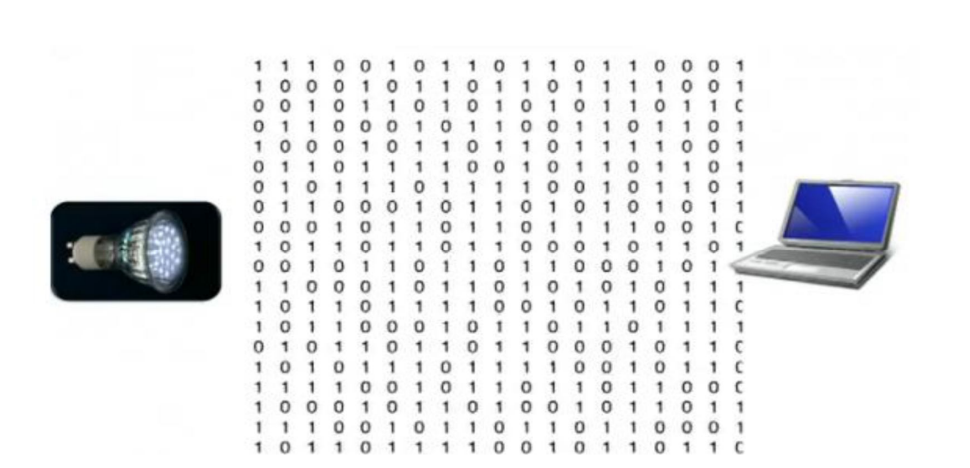
\includegraphics[scale=0.7]{banu.png}
\caption{Image 1}
\label{fig:LIFI}
\end{figure}


\chapter{SURVEY OF SIMILAR APPLICATION IN MARKET} 
Content
\linespread{1.5} 
 
%SEMINAR DESCRIPTION 
\chapter{FRAMEWORK DESCRIPTION} 
\linespread{1.5} 
\section{Frontend Implementation} 
\textbf{3.1.1 Environment Setup}

Content

\textbf{3.1.2 Structure of the Project}

Content

\textbf{3.1.3 Execution Procedure}

Content


\section{Backend Implementation} 

\textbf{3.2.1 Environment Setup}

Content

\textbf{3.2.2 Structure of the Project}

Content

\textbf{3.2.3 Execution Procedure}
Content


\begin{figure}[h]
\centering
\includegraphics[scale=1]{sample 3.png}
\caption{Image 2}
\label{fig:LIFI}
\end{figure}



\section{Database Implementation} 
\textbf{3.3.1 Database Configuration}

Content

\textbf{3.1.2 Schema Structure}

Content

\textbf{3.1.3 Tables created}

Content

\chapter{ METHODOLOGIES } 
\linespread{1.5} 
\section{Project Architecture} 
  
content

\section{DataFlow Diagram} 
Content 

\section{Module 1:} 
Content 

\section{Module 2:} 
Content 

\section{Module 3:} 
Content 

\textbf{Advantages of this Project} 

Content

 \textbf{a) Title 1:} content
 
\textbf{b) Title 2:} Content

\textbf{c) Title 3:} Content


\textbf{Disadvantages} 

Content
\chapter{RESULTS AND DISCUSSIONS} 
\linespread{1.5} 
Content with screenshots
\\

\begin{table}[h!]
  \begin{center}
    \caption{ Example Comparison}
    \label{tab:Speed Comparision}
    \begin{tabular}{l|c} 
      \textbf{Applications} & \textbf{Advantages}\\
      
      \hline
      Wi-Fi - IEEE 802.11n & ~150Mbps\\
      IrDA & ~1Mbps\\
      Bluetooth & 3Mbps\\
      NFC & 124Kbps\\
      Li-Fi & ~ 1Gbps
    \end{tabular}
  \end{center}
\end{table}\\

\begin{figure}[h]
\centering
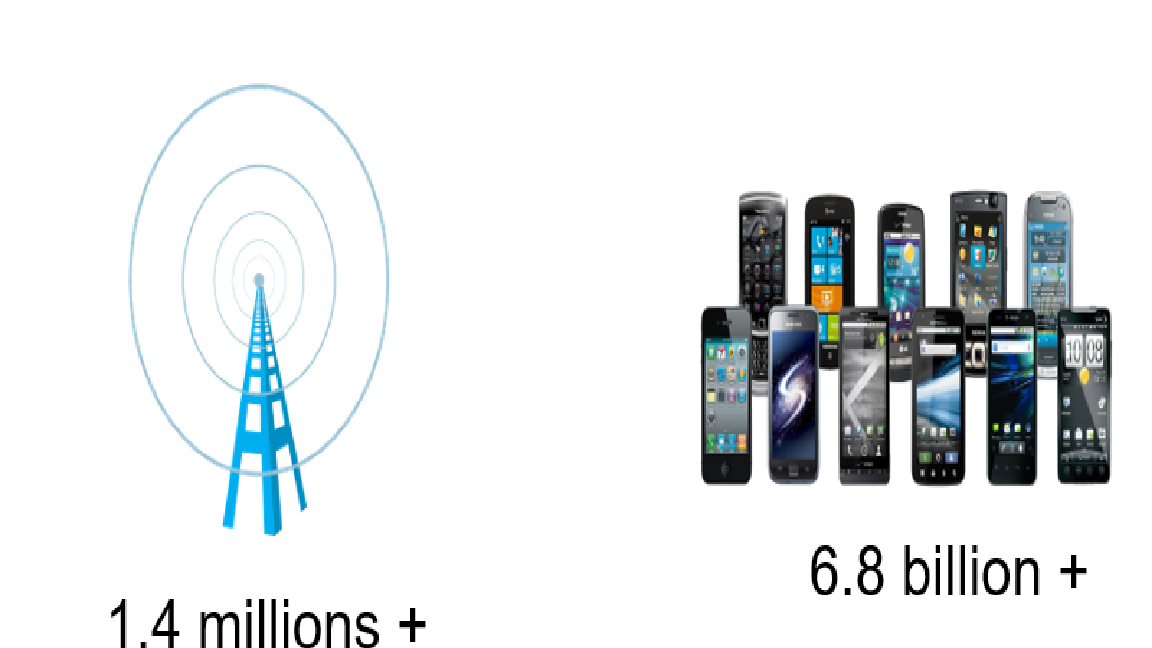
\includegraphics[scale=0.7]{banu 4.png}
\caption{Image 3}
\label{fig:LIFI}
\end{figure} \\

\\





\chapter{CONCLUSION AND FUTURE ENHANCEMENTS} 
\linespread{1.5} 
\section{Conclusion} 
content

 
\section{Future Enhancements} 
Content

 
\addcontentsline{toc}{chapter}{References} 
\renewcommand\bibname{References} 
 
Contents about Existing Applications and Review Comments (add link of the applications too)


\end{document}
